\subsection{Модуль распознавания лиц}

Данный модуль состоит из трех несвязных частей -- распознавания лиц
в видеопотоке, распознавания лиц со статичного изображения, детектирования лиц
со статичного фото.

\subsubsection{Детектирование лиц со статичного изображения}

Для разработки функции детектирования лиц использовался алгоритм, основанный на
методе Виолы-Джонса. Данный метод основывается на примитивах Хаара,
представляющих собой разбивку заданной прямоугольной области на наборы
разнотипных прямоугольных подобластей:

\addimghere{haar-cascade}{0.8}{примитивы Хаара}

Для того, чтобы найти лицо, нужно выделить его основные компоненты, такие как
нос, глаза, лоб, губы. Для этого существуют специальные шаблоны (примитивы)
Хаара:

\addimghere{haar-cascade-eyes}{0.8}{примитивы Хаара для: лба, носа, глаз, губ,
подбородка (слева направо)}

Для каждого из этих шаблонов, высчитывается разность между яркостью белой
и чёрной областей. Это значение сравнивается с эталоном и принимается решение
о том, найдено лицо на фото или нет. В этом заключается метод Виолы-Джонса,
который успешно используется в сфере компьютерного зрения.

\addimghere{viola-jones-example}{0.4}{пример использования шаблонов Хаара}

Библиотека распознавания OpenCV имеет свою имплементацию алгоритма
Виолы-Джонса, использование заключается в написании следующего кода:

\lstset{language=Python, basicstyle=\normalsize, keepspaces=true, numbers=left, breaklines=true,
frame=single, showstringspaces=true, columns=fullflexible} 
\begin{lstlisting}
import cv2 as cv

face_cascade = cv.CascadeClassifier('haarcascade.xml')
faces = face_cascade.detectMultiScale(#COLOR, 3, 5)
\end{lstlisting}

%% TODO: image as numpy array

Создание класса \textit{CascadeClassifier} происходит на основе файла с шаблонами
(примитивами) в формате XML. Данный класс содержит функцию
\textit{detectMultiScale()}, которая выполняет предобработку изображения --
преобразует его в черно-белый цвет и выполняет базовую цветокоррекцию, что
позволяет увеличить эффективность детектирования. После предобработки функция
применяет метод Виолы-Джонса, и возвращает результат в виде массива
с координатами лица на изображении. 

\subsubsection{Распознавание лиц со статического изображения}

Распознавание лица - это идентификация личности человека с заданного
изображения на основе имеющихся баз данных. Технология распознавания требует
минимум два этапа:

\begin{itemize*}
\item "обучение" системы на конкретные лица или массив лиц;
\item распознавание на основе "обучающих" данных.
\end{itemize*}

Под термином "обучение" в данном случае подразумевается преобразование
изображения в вид, удобный и эффективный для сравнения.
Для решения данной задачи использовался алгоритм Local Binary Patterns (LBP).
Данный алгоритм состоит из следующих этапов:

\begin{itemize*}
  \item разделить изображение на части;
  \item в каждой части интенсивность цвета центрального пикселя сравнивается
    с интенсивностью соседних пикселей;
  \item если значение центрального больше соседнего, соседний пиксель
    заменяется на 0, иначе на 1. В результате получается некоторое число (см.
    Рисунок 23);
  \item на основе полученного числа строится гистограмма;
  \item гистограммы всех частей объединяется в один вектор, характеризующий
    изображение в целом. Такой числовой вектор можно использовать для сравнения
    и хранить в базе данных.
\end{itemize*}

\addimghere{thresholding}{0.7}{Вычисление числа части изображения}
\addimghere{histogram}{0.6}{Вычисление общей гистограммы и построение вектора}

В библиотеке Face Recognition использовать алгоритм Local Binary Patterns можно следующим
образом:

\begin{lstlisting}
import cv2 as cv
import face_recognition

# Вычисление вектора полученного изображения
# IMAGE - изображение, COORDINATES - координаты найденного лица
encodings = face_recognition.face_encodings(IMAGE, COORDINATES)

# Сравнение полученного вектора с имеющимся в базе
# В случае распознавания функция вернёт значение True, иначе False
matches = face_recognition.compare_faces(knownEncodings, encoding)
\end{lstlisting}

\subsubsection{Тренировка распознавания системы}

Модуль распознавания требует наличия базы данных с лицами. Для каждого
человека, которому должен быть разрешён доступ, нужно создать запись в базе
данных с числовым вектором тренировочного фото, для дальнейшего сравнивания
с кадрами из видеопотока. 

Для решения задачи использовалась библиотека pickle -- это база данных,
основанная на файлах, и хранящая информацию в виде "ключ - значение". Подобный
формат хранения удобно использовать для тренировки системы распознавания --
достаточно получить числовой вектор лица, и сохранить в базе данных в виде "имя
- вектор". 

\begin{lstlisting}
import pickle

# Чтение базы данных из файла
# PATH - путь хранения файла
data = pickle.loads(open(PATH, "rb").read())

# Получение из базы данных массива имён и массива векторов
knownEncodings = data["encodings"]
knownNames = data["names"]

# Формирование словаря (ассоциативный массив)
# и сохранение в базу данных
data = {"encodings": knownEncodings, "names": knownNames}
f = open(PATH, "wb")
f.write(pickle.dumps(data)).close()
\end{lstlisting}

\subsubsection{Распознавание лиц с видеопотока}

Используя детектирование и распознавание лиц был разработан модуль,
описываемый в данной главе. Алгоритм работы модуля заключается в использования
видеопотока с камеры с помощью библиотеки picamera,

\begin{lstlisting}
import picamera 
from picamera import VideoStream

stream = picamera.VideoStream(0)
while True:
  # Получение кадров с камеры в бесконечном потоке
  (ret, frame) = stream.read()
\end{lstlisting}
и сравнивании изображения с потока с изображениями из базы данных. 

\newpage

\begin{figure}[h!]
  \centering
  \setlength{\fboxsep}{5pt}
  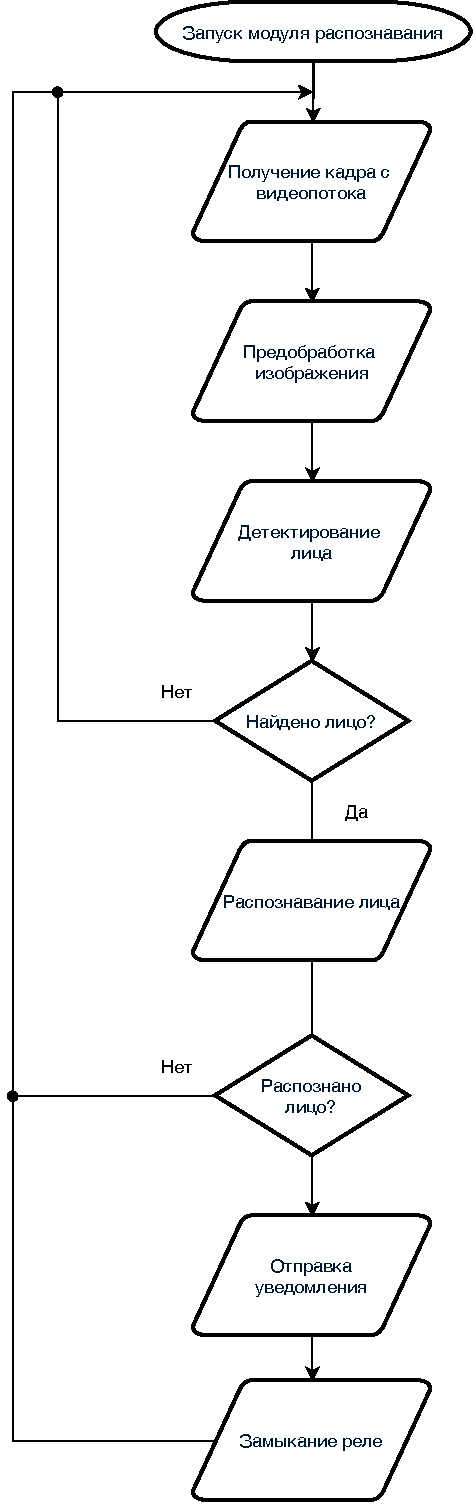
\includegraphics[width=0.4\textwidth]{data-visualisation/image-processing}
  \vspace*{6pt}
  \caption{Алгоритм работы модуля распознавания}\label{fig:image-processing}
\end{figure}
